%%%%%%%% ICML 2025 EXAMPLE LATEX SUBMISSION FILE %%%%%%%%%%%%%%%%%

\documentclass{article}

% Recommended, but optional, packages for figures and better typesetting:
\usepackage{microtype}
\usepackage{graphicx}
\usepackage{subfigure}
\usepackage{booktabs} % for professional tables

\usepackage{physics}
\usepackage{mhchem}
\usepackage{bm}
\usepackage{mathtools}
\usepackage{algorithm}
\usepackage{algorithmic}

% hyperref makes hyperlinks in the resulting PDF.
% If your build breaks (sometimes temporarily if a hyperlink spans a page)
% please comment out the following usepackage line and replace
% \usepackage{icml2025} with \usepackage[nohyperref]{icml2025} above.
\usepackage{hyperref}


% Attempt to make hyperref and algorithmic work together better:
\renewcommand{\theHalgorithm}{\arabic{algorithm}}

% Use the following line for the initial blind version submitted for review:
\usepackage[accepted]{icml2025}

% If accepted, instead use the following line for the camera-ready submission:
% \usepackage[accepted]{icml2025}

% For theorems and such
\usepackage{amsfonts}
\usepackage{amsmath}
\usepackage{amssymb}
\usepackage{mathtools}
\usepackage{amsthm}
\usepackage{thmtools}
\usepackage{thm-restate}

% if you use cleveref..
\usepackage[capitalize,noabbrev]{cleveref}

%%%%%%%%%%%%%%%%%%%%%%%%%%%%%%%%
% THEOREMS
%%%%%%%%%%%%%%%%%%%%%%%%%%%%%%%%
\theoremstyle{plain}
\newtheorem{theorem}{Theorem}[section]
\newtheorem{proposition}[theorem]{Proposition}
\newtheorem{lemma}[theorem]{Lemma}
\newtheorem{corollary}[theorem]{Corollary}
\theoremstyle{definition}
\newtheorem{definition}[theorem]{Definition}
\newtheorem{assumption}[theorem]{Assumption}
\theoremstyle{remark}
\newtheorem{remark}[theorem]{Remark}

% Todonotes is useful during development; simply uncomment the next line
%    and comment out the line below the next line to turn off comments
%\usepackage[disable,textsize=tiny]{todonotes}
\usepackage[textsize=tiny]{todonotes}

% enable \mathscr
\usepackage{mathrsfs}

% define SE(3), SO(3) and IGSO(3) in math mode
\DeclareMathOperator{\SE}{SE}
\DeclareMathOperator{\SO}{SO}
\DeclareMathOperator{\IGSO}{IGSO}
\DeclareMathOperator{\se}{\mathfrak{se}}
\DeclareMathOperator{\so}{\mathfrak{so}}
\DeclareMathOperator{\igso}{\mathfrak{igso}}

% define \Exp and \Log for Lie groups
\DeclareMathOperator{\Exp}{\operatorname{Exp}}
\DeclareMathOperator{\Log}{\operatorname{Log}}

% define \argmax and \argmin
\DeclareMathOperator*{\argmax}{arg\,max}
\DeclareMathOperator*{\argmin}{arg\,min}

% define \R \N \Z \C
\DeclareMathOperator{\R}{\mathbb{R}}
\DeclareMathOperator{\N}{\mathbb{N}}
\DeclareMathOperator{\Z}{\mathbb{Z}}
\DeclareMathOperator{\C}{\mathbb{C}}
\DeclareMathOperator{\Q}{\mathbb{Q}}
\DeclareMathOperator{\F}{\mathbb{F}}

% define \P \E
\let\P\relax
\DeclareMathOperator{\P}{\mathbb{P}}
\DeclareMathOperator{\E}{\mathbb{E}}

% define stop-grad
\DeclareMathOperator{\sg}{\mathrm{sg}}

% define iid \sim
\DeclareMathOperator{\iid}{\overset{\mathrm{i.i.d.}}{\sim}}

\newcommand{\inner}[2]{\left\langle #1, #2\right\rangle}

% The \icmltitle you define below is probably too long as a header.
% Therefore, a short form for the running title is supplied here:
\icmltitlerunning{Fine-tuning BioEmu}

\begin{document}

\twocolumn[
    \icmltitle{Fine-tuning BioEmu for Accurate Protein Folding Stability Prediction}

    \icmlsetsymbol{equal}{*}

    \begin{icmlauthorlist}
        \icmlauthor{Zhaoyang Li}{equal,zhaoyangli}
        % \icmlauthor{Brian L. Trippe}{equal,btrippe}
    \end{icmlauthorlist}

    \icmlaffiliation{zhaoyangli}{Department of Bioengineering, Stanford University, CA 94305, USA}
    % \icmlaffiliation{btrippe}{Department of Statistics, Stanford University, CA 94305, USA}

    \icmlcorrespondingauthor{Zhaoyang Li}{zhaoyangli@stanford.edu}
    % \icmlcorrespondingauthor{Brian L. Trippe}{btrippe@stanford.edu}

    \icmlkeywords{Machine Learning, ICML}

    \vskip 0.3in
]

\printAffiliationsAndNotice{\icmlEqualContribution} % otherwise use the standard text.

\begin{abstract}
    Recent advances in protein structure prediction models such as AlphaFold have largely resolved static folding problems. However, accurately profiling dynamic protein conformations to estimate folding stabilities remains a huge challenge.
    Biomolecular Emulator (BioEmu) is a recent generative deep learning framework that employs a Property Prediction Fine-Tuning (PPFT) algorithm that integrates extensive MEGAScale experimental datasets with molecular dynamics (MD) simulations to infer folding free energies. Despite its innovative design, preliminary fine-tuning results revealed limitations in predictive accuracy.
    In this work, we propose a novel approach that efficiently fine-tunes a $\SE(3)$ equivariant diffusion model using experimental expectation values, while preserving the majority of the pretrained parameters to maintain the integrity of the underlying diffusion process. This work may mark a significant advance in the integration of experimental data with deep generative models, paving the way for more reliable computational assessments of protein folding energy landscapes.
\end{abstract}

\section{Introduction}

Predicting protein stability (e.g.\ folding free energy changes $\Delta\Delta G$) from sequence and limited structural information is a long-standing challenge. Biomolecular Emulator (BioEmu) is a recently proposed generative diffusion model that addresses this by emulating protein conformational ensembles and integrating experimental stability data~\cite{bioemu}. In BioEmu's original framework, a property-prediction fine-tuning (PPFT) algorithm was used to incorporate experimental stability measurements without requiring known structures. PPFT works by generating a small ensemble of structures (using a fast $8$-step diffusion sampling) and comparing an observable (fraction of folded structures) to experimental values, then backpropagating the error to adjust the model. This strategy enabled BioEmu to predict stability with high accuracy, outperforming black-box sequence-based models.

However, the PPFT approach has limitations: it introduces an approximation in sampling that may perturb the pretrained distribution, and it does not explicitly account for the geometrical symmetries of protein conformations. Recent advances in $\SE(3)$ equivariant diffusion modeling provide a more principled framework for generative processes on the manifold of rigid-body transformations~\cite{se3_diffusion}. Our central idea is to reinterpret fine-tuning as a constrained optimization on the manifold of protein conformations, where we impose that certain expected observables match experimental values while minimally perturbing the pretrained ensemble distribution. This project will pursue that idea in four stages, each serving as an independent milestone:

\section{Prototype $\IGSO(3)$ Diffusion on $\SO(3)$}

The first milestone is to prototype an isotropic Gaussian $\SO(3)$ ($\IGSO(3)$) diffusion process using a toy problem~\cite{so3_diffusion}. We begin with a simple synthetic distribution on $\SO(3)$ that contains $K$ $\IGSO(3)$ components with different mean rotations, variances, and mixture weights. The goal is to train a simple neural network to learn the score function (Proposition~\ref{prop:stein_score}) and model the distribution through reverse diffusion sampling (Algorithm~\ref{alg:em_predictor_so3}). Results is visualized by plotting the sampled marginal distribution of the rotation angle $\omega$ (Proposition~\ref{prop:marginal_igso3}).

Here we (i) formulate the forward and reverse stochastic differential equations (SDEs) on $\SO(3)$~\cite{riemannian_diffusion,sde_on_manifolds_hsu}
(ii) parameterizing $\SO(3)$ diffusion with the axis-angle representation of rotation~\cite{micro_lie_theory} and (iii) train a neural network $s_\theta(\mathbf{R}_t, t) \in \R^3$ via denoising score matching~\cite{score_based_diffusion}.

\begin{figure}[!ht]
    \centering
    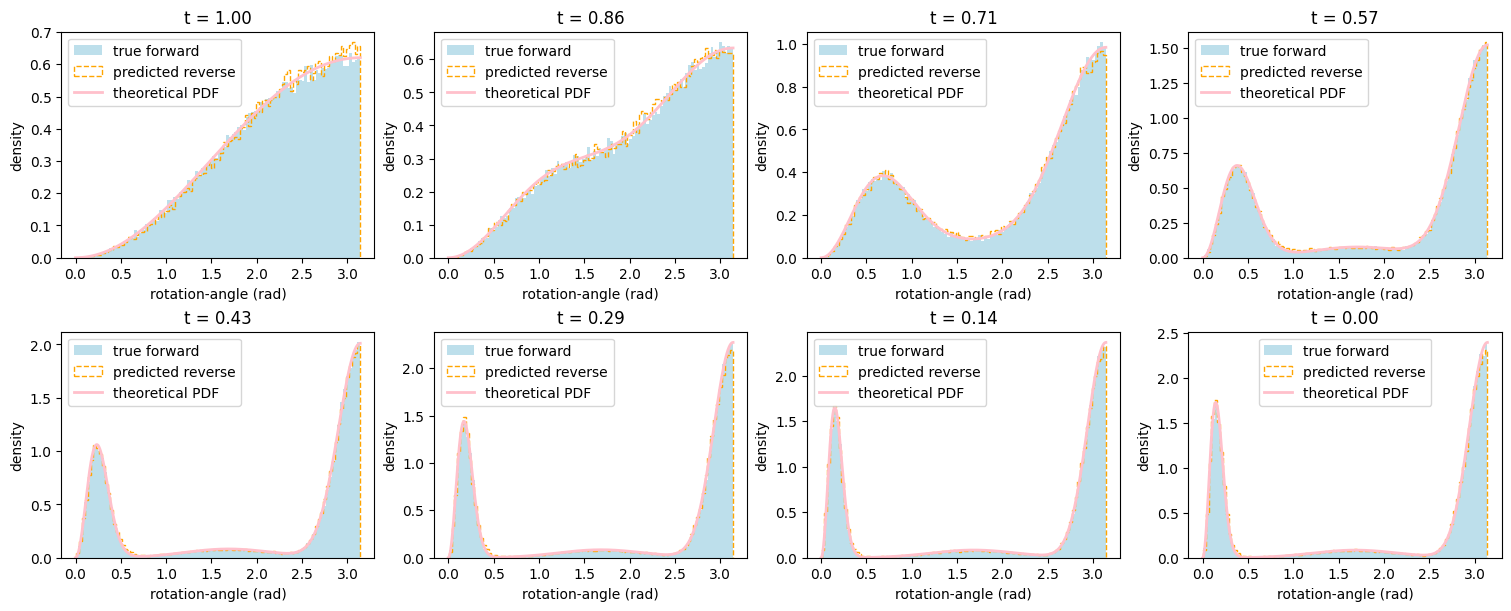
\includegraphics[width=\linewidth]{figures/train_visualization.png}
    \caption{Learned marginal densities of the rotation angle $\omega$ for a three-component $\IGSO(3)$ mixture, evaluated at eight evenly spaced noise levels $t\in\qty{1.00,0.86,\dots,0.00}$. The orange dashed lines are the predicted reverse histograms, while the blue shading is the true forward samples. The solid pink line is the theoretical PDF given by Proposition~\ref{prop:marginal_igso3}.}
    \label{fig:train_visualization}
\end{figure}

Figure~\ref{fig:train_visualization} shows the learned marginal densities of the rotation angle $\omega$ for an $\IGSO(3)$ mixture of identity, rotation by $\frac{\pi}{2}$ along the $y$-axis, and rotation by $\pi$ along the $z$-axis. At the start of the reverse process ($t=1.00$), the forward-perturbed distribution is essentially the uniform Haar measure on $\SO(3)$, and the network's predicted reverse histogram (orange dashed) overlaps almost perfectly with the true forward samples (blue shading).

As $t$ decreases, the marginals collapse onto the two sharp peaks at $\omega\approx0$ and $\omega\approx\pi$, as well as a third broad peak at $\omega\approx\frac{\pi}{2}$, which matches the original three-component mixture up to sampling noise. Across every time slice, the predicted reverse densities lie almost exactly on top of the theoretical PDF (solid red), which builds confidence in applying similar $\SE(3)$ equivariant diffusion principles to protein models.

\section{Fine-tuning BioEmu Demonstration on a Single Protein}

Next, we apply the new fine-tuning method (Proposition~\ref{prop:diffusion_model_finetune}) on the $\IGSO(3)$ mixture case. We use the same $\IGSO(3)$ mixture model as above, but add a constraint that the expected value of mixture weights $\E_{\mathbf{R}_0\sim\IGSO(3)}[h_i(\mathbf{R}_0)]$ matches some slightly different values $h_i^*$, where $h_i(\mathbf{R}_0)$ is the $i$-th observable of the mixture model (Proposition~\ref{prop:unbiasedness}).

\begin{figure}[!ht]
    \centering
    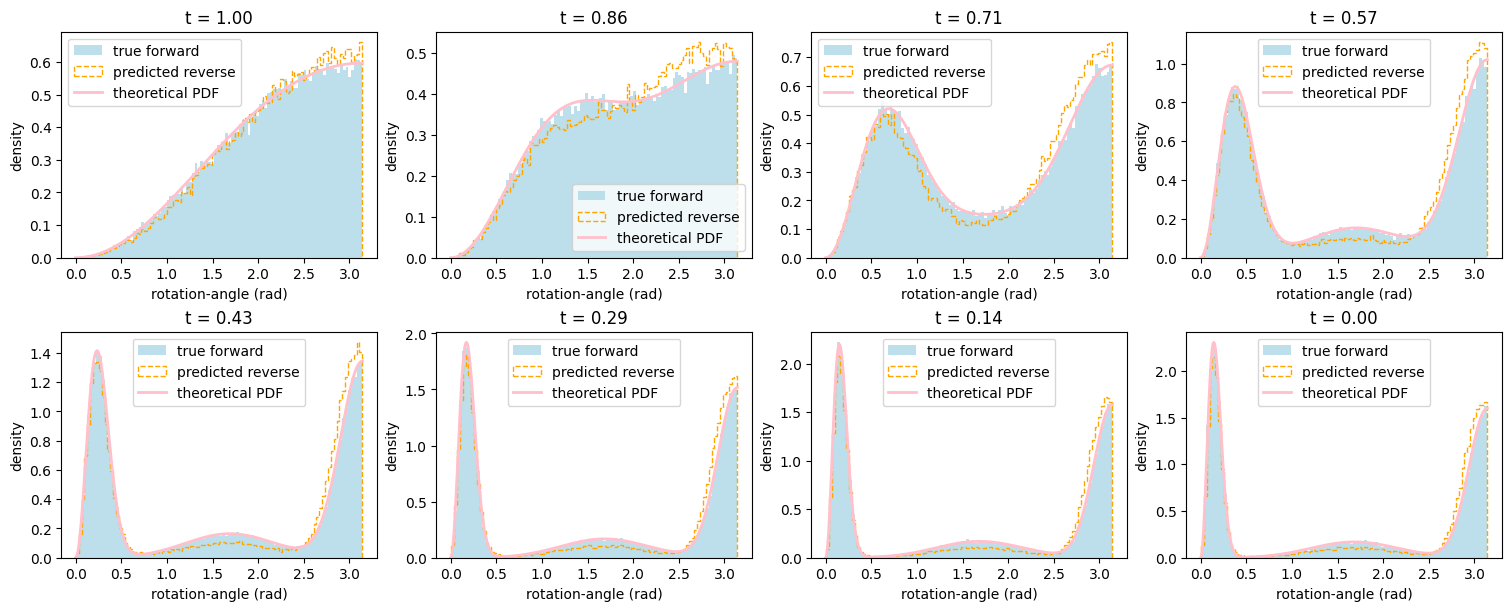
\includegraphics[width=\linewidth]{figures/finetune_visualization.png}
    \caption{Fine-tuned marginal densities of the rotation angle $\omega$ for the $\IGSO(3)$ mixture. Legends remains the same as Figure~\ref{fig:train_visualization}.}
    \label{fig:finetune_visualization}
\end{figure}

Figure~\ref{fig:finetune_visualization} shows the same set of marginal rotation-angle densities after fine-tuning the score network to satisfy the new mixture-weight constraints $h_i^*$. As we anneal down, The predicted reverse histogram overlaps the true forward samples better with their relative heights shifted in accordance with the target weights $h_i^*$, confirming that we realize the new mixture composition without retraining from scratch.

We will apply this approach on BioEmu for a single protein sequence to demonstrate a proof-of-concept in a real-world scenario. Prior to this, we will need to fine-tune the toy model of two $\IGSO(3)$ distributions to adjust their mixture weights.

Then we will select an example protein with an extreme stability phenotype. One candidate is an IDP from the CALVADOS dataset used in the BioEmu paper. Using this protein, our method will enforce this via the constrained optimization above. After fine-tuning on this single sequence, we expect that an IDP's generated conformations will be mostly unfolded, matching experimental observations.

\section{Scaling to MEGAScale Dataset and MD Data}

Having validated the approach on a single protein, we will extend it to a large-scale fine-tuning using the MEGAScale dataset of protein folding stabilities, which was also used in training the original BioEmu. For each protein or mutant in the training set, the model will generate an ensemble and compute an expected stability-related quantity. We will then compute the error between these model predictions and the experimental values, and update the model parameters to reduce this error. In addition to the experimental data, we will also attempt to incorporate the molecular dynamics (MD) simulation dataset to provide direct structural physics signals.

{\bf Milestone outcome:} a fine-tuned version of the BioEmu model that integrates experimental stability data via our SE(3) equivariant constrained fine-tuning method. This model should have hopefully improved accuracy (in terms of predicted vs experimental $\Delta\Delta G$) while retaining physically plausible conformational sampling.

\section{Benchmarking and Evaluation}

The final stage focuses on rigorous evaluation of the fine-tuned model against benchmarks, and comparison to the original PPFT-based BioEmu. We will use the same evaluation protocols and datasets as the original BioEmu study to ensure a direct comparison.
First, on the held-out stability dataset, we will assess the predictive $\Delta\Delta G$ accuracy of our model.
Next, we will evaluate if our model has preserved the pretrained distribution aside from the intended shifts in stability-related aspects. For example, we will apply our fine-tuned model to sample ensembles for proteins with known conformational changes or binding events to verify that it still generates diverse, biologically relevant conformations.
Finally, we will compare our model’s predictions to other computational stability predictors such as single-point mutations with known experimental $\Delta\Delta G$ (ProTherm or the SKEMPI database) and see how well our model’s predicted stability change correlates with experiments.

{\bf Milestone outcome:} a comprehensive benchmark report. We expect to show that our SE(3) equivariant fine-tuning method achieves at least comparable accuracy to PPFT on stability prediction, and we will highlight any improvements.

\section{Related Work}

\section{Experiment}

\section{Discussion}

\section*{Acknowledgements}

% In the unusual situation where you want a paper to appear in the
% references without citing it in the main text, use \nocite
% \nocite{bioemu}

\bibliography{example_paper}
\bibliographystyle{icml2025}


%%%%%%%%%%%%%%%%%%%%%%%%%%%%%%%%%%%%%%%%%%%%%%%%%%%%%%%%%%%%%%%%%%%%%%%%%%%%%%%
%%%%%%%%%%%%%%%%%%%%%%%%%%%%%%%%%%%%%%%%%%%%%%%%%%%%%%%%%%%%%%%%%%%%%%%%%%%%%%%
% APPENDIX
%%%%%%%%%%%%%%%%%%%%%%%%%%%%%%%%%%%%%%%%%%%%%%%%%%%%%%%%%%%%%%%%%%%%%%%%%%%%%%%
%%%%%%%%%%%%%%%%%%%%%%%%%%%%%%%%%%%%%%%%%%%%%%%%%%%%%%%%%%%%%%%%%%%%%%%%%%%%%%%
\newpage
\appendix
\onecolumn

\section{Preliminaries and Notation}

Throughout this paper we adopt the following notation and conventions.

\paragraph{Manifolds and Lie groups.}
Let $\mathcal{M}$ denote a smooth, $d$-dimensional Riemannian manifold with metric $\inner{\cdot}{\cdot}_{\mathcal{M}}$ and associated volume form $\dd V$. $\mathbf{X} \in \mathcal{M}$ is a point on the manifold. We write $\SO(3)$ for the group of $3\times3$ rotation matrices and $\so(3)$ for its Lie algebra, and similarly $\SE(3)\cong\SO(3)\ltimes\R^3$ with Lie algebra $\se(3)=\so(3)\oplus\R^3$.

For any Lie group $G$ and its Lie algebra $\mathfrak{g}$, $\exp:\mathfrak{g}\to G$ is the Riemannian exponential map, and $\log:G\to\mathfrak{g}$ its (local) inverse. The isomorphism hat $[\cdot]^\wedge:\R^d \to\mathfrak{g}$ and vee $[\cdot]^\vee:\mathfrak{g}\to\R^d$, i.e.\ the vectorization and de-vectorization maps, induce $\Exp:\R^d\to G$ and $\Log:G\to\R^d$ by the composition of mappings, respectively.

The left action of $g\in G$ on $h\in G$ is $L_g(h)=gh$ and its differential is $\dd L_g: T_hG\to T_{gh}G$. The metric on $\SE(3)$ is given by the canonical left-invariant metric, which is induced by the standard inner product on $\so(3)$ and $\R^3$, i.e.\ $\inner{\mathbf{t}_1}{\mathbf{t}_2}_{\SE(3)}=\inner{\mathbf{x}_1}{\mathbf{x}_2}_{\R^3}+\inner{\mathbf{r}_1}{\mathbf{r}_2}_{\SO(3)}$ for $\mathbf{t}_1 =(\mathbf{r}_1,\mathbf{x}_1) \in \se(3)$ and $\mathbf{t}_2 =(\mathbf{r}_2,\mathbf{x}_2) \in \se(3)$. The bi-invariant Riemannian metric on $\SO(3)$ is given by its Killing form $\inner{\mathbf{r}_1}{\mathbf{r}_2}_{\SO(3)}=\frac{1}{2}\mathrm{tr}(\mathbf{r}_1^\mathrm{T}\mathbf{r}_2)$, where $\mathbf{r}_1,\mathbf{r}_2\in\so(3)$.

\paragraph{Protein backbone frames.}
A protein backbone of $N$ residues is represented by a sequence of rigid frames
\begin{equation*}
    \mathbf{T} = (\mathbf{T}_1,\dots,\mathbf{T}_N) \in \SE(3)^N,
    \quad \mathbf{T}_n=(\mathbf{R}_n,\mathbf{x}_n)
\end{equation*}
where $\mathbf{R}_n\in\SO(3)$ is the rotation matrix and $\mathbf{x}_n\in\R^3$ is the translation vector for residue $n$.
Each frame acts on the idealized residue coordinates $(\ce{N}^*,\ce{C}^*,\ce{C_\alpha}^*)\subset\R^3$ via
$\mathbf{T}_n(v)=\mathbf{R}_n v+\mathbf{x}_n$, so that the atomic positions for residue $n$ are
\begin{equation*}
    (\ce{N}_n,\ce{C}_n,{\ce{C_\alpha}}_n)=\mathbf{T}_n (\ce{N}^*,\ce{C}^*,\ce{C_\alpha}^*),
\end{equation*}
and the \ce{O} atom is placed by an additional torsion angle $\psi_n$ around the \ce{C_\alpha-C} bond.

\paragraph{Distributions on Lie groups.}
We denote the isotropic Gaussian distribution on $\SO(3)$ as $\IGSO(3)(\mathbf{R}_0, \sigma^2)$, where $\mathbf{R}_0$ is the mean rotation and $\sigma^2$ is the variance. The probability density function (PDF) of $\mathbf{R}_t \sim \IGSO(3)(\mathbf{R}_0, \sigma^2)$ when $t=\sigma^2$ is given by
\begin{equation}
    p(\mathbf{R}_t;\mathbf{R}_0, \sigma) = \frac{1}{8\pi^2}\sum_{\ell=0}^{\infty} (2\ell+1)e^{-\frac{\sigma^2}{2}\ell(\ell+1)}\chi_\ell(\mathbf{R}_0^\mathrm{T}\mathbf{R}_t)
\end{equation}
with respect to the canonical Haar measure on $\SO(3)$, $\mu_{\SO(3)} = 4\sin^2\frac{\omega}{2}\dd\omega\wedge\dd\varOmega$. Here $\chi_\ell$ is the $\ell$-th irreducible unitary representation of dimension $2\ell+1$ and $\varOmega$ is the solid angle on $\mathbb{S}^2$. The axis-angle representation $\mathbf{q} = \Log(\mathbf{R})$ and $\omega = \norm{\mathbf{q}}_2$ is used to describe the rotation for score matching. A random variable $\mathbf{R}_t\sim\IGSO(3)(\mathbf{R}_0, \sigma^2)$ is sampled from $\mathbf{R}_0\IGSO(3)(\mathbf{I}, \sigma^2)$, where $\mathbf{I}$ is the identity matrix.

\paragraph{Diffusion on manifolds.}
Let $\mathbf{X}_t$ be a diffusion process on manifold $\mathcal{M}$ with drift $b(\mathbf{X}_t, t)$ and diffusion $g(t)$. We consider time $t\in[0, 1]$ and a forward and reverse It\^o SDE on $\mathcal{M}$:
\begin{align}
    \dd\mathbf{X}_t & = b(\mathbf{X}_t, t) \dd t + g(t) \dd \mathbf{W}_t^\mathcal{M}                                                             \\
    \dd\mathbf{X}_t & = \qty(b(\mathbf{X}_t, t) - g(t)^2 \nabla_{\mathbf{X}_t} \log p_t(\mathbf{X}_t)) \dd t + g(t) \dd \mathbf{W}_t^\mathcal{M}
\end{align}
where $\mathbf{W}_t^\mathcal{M}$ is Brownian motion on $\mathcal{M}$. This gives the same form as the standard Stratonovich SDE typically used on manifolds, as the diffusion term does not depend on the state $\mathbf{X}_t$. The time-reversed process requires the Stein score $\nabla_{\mathbf{X}_t} \log p_t(\mathbf{X}_t)$, which is the Riemannian gradient of the log-density.

\paragraph{Fine-tuning diffusion models.}
Suppose we introduce an additional drift term $u(\tilde{\mathbf{X}}_t, t)$ into the original reverse diffusion process:
    \begin{equation}
        \begin{aligned}
            \dd\tilde{\mathbf{X}}_t ={} &
            \qty(b(\tilde{\mathbf{X}}_t, t)
            - g(t)^2\nabla_{\tilde{\mathbf{X}}_t}\log p_t(\mathbf{X}_t))\dd t   \\
                                        & + g(t)u(\tilde{\mathbf{X}}_t, t)\dd t
            + g(t)\dd \mathbf{W}_t^\mathcal{M}
        \end{aligned}
    \end{equation}
    and solve the following constrained optimization problem:
    \begin{equation}
        \begin{aligned}
            & \argmin_{u} D_\text{KL}(\tilde{\mathbf{X}}_0\parallel \mathbf{X}_0)   \\
            \text{s.t.} \quad
            & \mathbb{E}_{\tilde{\mathbf{X}}_0}[h_i(\tilde{\mathbf{X}}_0)] = h_i^*,
            \quad i = 1,\dots,N\,.
        \end{aligned}
    \end{equation}

    We choose to minimize the Kullback-Leibler (KL) divergence between the original and perturbed distributions:
    \begin{equation}
        \begin{aligned}
            D_\text{KL}(\tilde{\mathbf{X}}_0\parallel \mathbf{X}_0) & \leq D_\text{KL}(\tilde{\P}\parallel \P) \\
            & = \frac{1}{2}\mathbb{E}_{\tilde{\P}} \qty[\int_0^1 \norm{u(\tilde{\mathbf{X}}_t, t)}_\mathcal{M}^2 \dd t]
        \end{aligned}
    \end{equation}
    hence the fine-tuning loss of the diffusion model is given by
    \begin{equation}
        \mathcal{L}(\theta) = \E_{\mathbf{X} \iid \P_{\sg(\theta)}}\qty[\hat{L}_\theta^\text{EV}(\mathbf{X}^{(1)}, \mathbf{X}^{(2)}, \dots, \mathbf{X}^{(M)}) + \lambda\hat{L}_\theta^\text{KL}(\mathbf{X}^{(1)}, \mathbf{X}^{(2)}, \dots, \mathbf{X}^{(M)})]
    \end{equation}
    where $\hat{L}_\theta^\text{EV}$ is the empirical variance loss and $\hat{L}_\theta^\text{KL}$ is the empirical KL divergence loss. We have also applied the leave-one-out estimator for the empirical KL divergence loss.

\section{Brownian Motion on Lie Groups}

\subsection{Marginal distribution and score function of $\IGSO(3)$}

\begin{proposition}[Marginal Distribution of $\IGSO(3)$]\label{prop:marginal_igso3}
    Let $\mathbf{R}_t \sim \IGSO(3)(\mathbf{R}_0, \sigma^2)$ be a random rotation matrix. The marginal distribution of its rotation angle $\omega_t = \norm{\Log(\mathbf{R}_t)}_2$ is given by its PDF $\frac{1-\cos\omega_t}{\pi}f(\omega_t; \mathbf{R}_0, \sigma)$, where $f(\omega_t; \mathbf{R}_0, \sigma)$ is defined as
    \begin{equation}
        f(\omega_t; \mathbf{R}_0, \sigma) = \sum_{\ell=0}^{\infty} e^{-\frac{\sigma^2}{2}\ell(\ell+1)}\frac{\sin\left(\ell+\frac{1}{2}\right)\omega_0}{\sin \frac{\omega_0}{2}}\frac{\sin\left(\ell+\frac{1}{2}\right)\omega_t}{\sin \frac{\omega_t}{2}}
    \end{equation}
    Here $\omega_0 = \norm{\Log(\mathbf{R}_0)}_2$ is the rotation angle of $\mathbf{R}_0$.
\end{proposition}

\begin{proof}
    The proof follows from the fact that the marginal distribution of $\omega_t$ is given by integrating the joint density against the Haar measure $\dd \mu_{\SO(3)} = 4\sin^2\frac{\omega}{2}\dd\omega\wedge\dd\varOmega$, constrained to rotations of fixed angle on $\mathbb{S}^2$:
    \begin{equation}
        \begin{aligned}
            \frac{1-\cos\omega_t}{\pi}f(\omega_t; \mathbf{R}_0, \sigma) & =4\sin^2\frac{\omega_t}{2}\int_{\mathbb{S}^2} p(\mathbf{R}_t; \mathbf{R}_0,\sigma) \dd\varOmega \\
             &= \frac{1-\cos\omega_t}{4\pi^2}\sum_{\ell=0}^{\infty} (2\ell+1)e^{-\frac{\sigma^2}{2}\ell(\ell+1)}\int_{\mathbb{S}^2} \chi_\ell(\mathbf{R}_0^\mathrm{T}\mathbf{R}_t) \dd\varOmega
        \end{aligned}
    \end{equation}
    where $\chi_\ell(\mathbf{R}_0^\mathrm{T}\mathbf{R}_t)$ denotes the $\ell$-th irreducible unitary representation of $2\ell+1$ dimension. Writing the character in terms of Wigner $D$-matrices:
    \begin{equation}
        \begin{aligned}
            \chi_\ell(\mathbf{R}_0^\mathrm{T}\mathbf{R}_t) & = \sum_{m=-\ell}^{\ell} D_{mm}^{(\ell)}(\mathbf{R}_0^\mathrm{T}\mathbf{R}_t) \\
            & = \sum_{m=-\ell}^{\ell} \sum_{n=-\ell}^{\ell} D_{mn}^{(\ell)}(\mathbf{R}_0) D_{nm}^{(\ell)}(\mathbf{R}_t) \\
            \end{aligned}
    \end{equation}
    
    Now consider integrating $D^{(\ell)}(\mathbf{R}_t)$ on $\mathbb{S}^2$. For any $\mathbf{R} \in \SO(3)$, the integral over the class of rotations sharing a given rotation angle is invariant under conjugation, which implies
    \begin{equation}
        \begin{aligned}
            \int_{\mathbb{S}^2} D^{(\ell)}(\mathbf{R}_t) \dd\varOmega & = \int_{\mathbb{S}^2} D^{(\ell)}(\mathbf{R}\mathbf{R}_t\mathbf{R}^{-1}) \dd\varOmega \\
            & = D^{(\ell)}(\mathbf{R})\qty(\int_{\mathbb{S}^2} D^{(\ell)}(\mathbf{R}_t) \dd\varOmega) D^{(\ell)}(\mathbf{R})^{-1} 
        \end{aligned}
    \end{equation}
    According to Schur's lemma, this integral must be proportional to the identity matrix, so we can write
    \begin{equation}
        \begin{aligned}
            \int_{\mathbb{S}^2} D^{(\ell)}(\mathbf{R}_t) \dd\varOmega & = \frac{1}{2\ell + 1} \tr\qty(\int_{\mathbb{S}^2} D^{(\ell)}(\mathbf{R}_t) \dd\varOmega) \mathbf{I} \\
            & = \frac{4\pi}{2\ell + 1} \chi_\ell(\mathbf{R}_t) \mathbf{I}
    \end{aligned}
    \end{equation}
    where $\mathbf{I}$ is the identity matrix. Thus, we can express the integral of $\chi_\ell(\mathbf{R}_0^\mathrm{T}\mathbf{R}_t)$ as
    \begin{equation}
        \begin{aligned}
            \int_{\mathbb{S}^2} \chi_\ell(\mathbf{R}_0^\mathrm{T}\mathbf{R}_t) \dd\varOmega & = \sum_{m=-\ell}^{\ell} \sum_{n=-\ell}^{\ell} D_{mn}^{(\ell)}(\mathbf{R}_0) \frac{4\pi}{2\ell + 1} \chi_\ell(\mathbf{R}_t) \delta_{mn} \\
            & = \frac{4\pi}{2\ell + 1} \chi_\ell(\mathbf{R}_t) \sum_{m=-\ell}^{\ell} D_{mm}^{(\ell)}(\mathbf{R}_0) \\
            & = \frac{4\pi}{2\ell + 1} \chi_\ell(\mathbf{R}_0) \chi_\ell(\mathbf{R}_t) \\
        \end{aligned}
    \end{equation}

    Substituting this back into the marginal distribution finally gives
    \begin{equation}
        \begin{aligned}
            f(\omega_t; \mathbf{R}_0, \sigma) & = \frac{1}{4\pi} \sum_{\ell=0}^{\infty} (2\ell + 1) e^{-\frac{\sigma^2}{2}\ell(\ell+1)}\int_{\mathbb{S}^2} \chi_\ell(\mathbf{R}_0^\mathrm{T}\mathbf{R}_t) \dd\varOmega \\
            & = \sum_{\ell=0}^{\infty} e^{-\frac{\sigma^2}{2}\ell(\ell+1)}\frac{\sin\left(\ell+\frac{1}{2}\right)\omega_0}{\sin \frac{\omega_0}{2}}\frac{\sin\left(\ell+\frac{1}{2}\right)\omega_t}{\sin \frac{\omega_t}{2}}
        \end{aligned}
    \end{equation}
\end{proof}

\begin{proposition}[Axis-Angle Decomposition of $\IGSO(3)$]\label{prop:axis_angle_decomposition}
    Let $\mathbf{R} = \mathbf{R}_0^\mathrm{T}\mathbf{R}_t$ be a random rotation matrix sampled from $\IGSO(3)(\mathbf{I}, \sigma^2)$ (so that $\mathbf{R}_{t} \sim \IGSO(3)(\mathbf{R}_0, \sigma^2)$). Let $\mathbf{q} = \Log(\mathbf{R})$ and $\omega = \norm{\mathbf{q}}_2$ be the axis-angle representation. Then the axis-angle decomposition of $\mathbf{R}$ is given by
    \begin{align}
        \frac{\mathbf{q}}{\omega} & \sim \mathcal{U}(\mathbb{S}^2)                             \\
        \omega                    & \sim \frac{1-\cos\omega}{\pi}f(\omega; \mathbf{I}, \sigma)
    \end{align}
    where $\mathcal{U}(\mathbb{S}^2)$ is the uniform distribution on the unit sphere $\mathbb{S}^2$.
\end{proposition}

\begin{proposition}[Score Function on $\SO(3)$]\label{prop:stein_score}
    Let $\mathbf{R}_0, \mathbf{R}_t\in\SO(3)$ and write their relative rotation as $\mathbf{R} = \mathbf{R}_0^\mathrm{T}\mathbf{R}_t$ with axis-angle representation $\mathbf{q}$ and $\omega$. Then the score function $s^*(\mathbf{q}, t) \in \R^3$ at time $t = \sigma^2$ of the reverse diffusion process satisfies
    \begin{equation}
        \begin{aligned}
            s^*(\mathbf{q}, t) & = \qty[\mathbf{R}_t^\mathrm{T} \nabla_{\mathbf{R}_t} \log p_t(\mathbf{R}_t\mid \mathbf{R}_0)]^\vee \\
                               & = \frac{\mathbf{q}}{\omega} \pdv{\omega} \log f(\omega; \mathbf{I}, \sigma)
        \end{aligned}
    \end{equation}
    where $p_t(\mathbf{R}_t\mid \mathbf{R}_0)$ is the conditional distribution of $\mathbf{R}_t$ given $\mathbf{R}_0$.
\end{proposition}

\subsection{Training and sampling SDEs on $\SO(3)$}

We aim to train a neural network to approximate the score function $s_\theta(\mathbf{R}_t, t)$ of the diffusion process on $\SO(3)$. The training objective is to minimize the denoising score matching loss:
\begin{equation}
    \argmin_\theta \mathbb{E}_{\mathbf{R}_0, \mathbf{R}_t\mid \mathbf{R}_0, t} \qty[\norm{\lambda(t) s_\theta(\mathbf{R}_t, t)-\lambda(t) s^*(\mathbf{q}, t)}^2_2]
\end{equation}
where $\lambda(t)$ is a time-dependent weighting function defined as the inverse of the standard deviation of the score function:
\begin{equation}
    \frac{1}{\lambda(t)} = \sqrt{\frac{1}{3}\E_{\mathbf{R}\sim \IGSO(3)(\mathbf{I}, \sigma)}\qty[\norm{s^*(\mathbf{q}, t)}_2^2]}
\end{equation}

The reverse sampling process is performed using the Euler-Maruyama method on $\SO(3)$. The algorithm is as follows:
\begin{algorithm}[!ht]
    \caption{Euler-Maruyama Predictor on $\SO(3)$}\label{alg:em_predictor_so3}
    \begin{algorithmic}[1]
        \REQUIRE SDE on $\SO(3)$ $\texttt{SO3SDE}$, score network $\texttt{ScoreNet}$, number of steps $N_\text{steps}$, noise weight $\lambda(t)$
        \ENSURE Sample $\mathbf{R}_0$
        \STATE $\qty{t_i}_{i=0}^{N_\text{steps}} \leftarrow \mathrm{linspace}(1, 0, N_\text{steps}+1)$
        \STATE $\Delta t \leftarrow \frac{1}{N_\text{steps}}$
        \STATE $\mathbf{R}_1 \sim \mathcal{U}(\SO(3))$
        \STATE $\mathbf{R} \leftarrow \mathbf{R}_1$
        \FOR{$i = 0$ {\bf to} $N_\text{steps}-1$}
        \STATE $t \leftarrow t_i$
        \STATE $s_\theta(\mathbf{R}, t) \leftarrow \texttt{ScoreNet}(\mathbf{R}, t)\cdot \frac{1}{\lambda(t)}$
        \STATE $(b(\mathbf{R}, t),g(t)) \leftarrow \texttt{SO3SDE}(\mathbf{R}, t)$
        \STATE $b(\mathbf{R}, t) \leftarrow b(\mathbf{R}, t) - g(t)^2 s_\theta(\mathbf{R}, t)$
        \STATE $z \sim \mathcal{N}(0, \mathbf{I})$
        \STATE $\mathbf{R} \leftarrow \mathbf{R} \Exp\qty(b(\mathbf{R}, t)\Delta t)$
        \STATE $\mathbf{R} \leftarrow \mathbf{R} \Exp\qty(g(t)z\sqrt{\Delta t})$
        \ENDFOR
        \STATE $\mathbf{R}_0 \leftarrow \mathbf{R}$
        \RETURN $\mathbf{R}_0$
    \end{algorithmic}
\end{algorithm}

\section{Fine-tuning diffusion models on Riemannian manifolds}

\subsection{Unbiased estimators for loss and gradients}

\begin{lemma}[Measure Transformation]\label{lem:measure_transformation}
    Let $h^{(1)}, h^{(2)}, \dots, h^{(M)} \in \R$ be a set of independent samples from the distribution $\Q_\theta$. Consider another distribution $\Q_\theta'$ which has a Radon-Nikodym derivative $w_\theta(h^{(i)}) = \frac{\dd \Q_\theta}{\dd \Q_\theta'}(h^{(i)})$. Then a loss function estimator $\hat{l}\qty(h^{(1)}, h^{(2)}, \dots, h^{(M)})$ with continuous second-order partial derivatives satisfies
    \begin{equation}
        \label{eq:measure_transformation}
        \E_{h\iid \Q_\theta}\qty[\hat{l}\qty(h^{(1)}, h^{(2)}, \dots, h^{(M)})] = \E_{h\iid \Q_\theta'}\qty[\hat{l}\qty(w_\theta(h^{(1)})h^{(1)}, w_\theta(h^{(2)})h^{(2)}, \dots, w_\theta(h^{(M)})h^{(M)})]
    \end{equation}
    if for all $i=1,\dots,M$,
    \begin{equation}
        \pdv[2]{\hat{l}}{{h^{(i)}}} = 0
    \end{equation}
\end{lemma}

\begin{proof}
    Assume $\pdv[2]{\hat{l}}{{h^{(i)}}} = 0$. The loss function should be able to be written as
    \begin{equation}
        \hat{l}\qty(h^{(1)}, h^{(2)}, \dots, h^{(M)}) = C_1^{(i)}\qty(h^{(1)}, \dots, h^{(i-1)}, h^{(i+1)}, \dots, h^{(M)}) h^{(i)} + C_2^{(i)}\qty(h^{(1)}, \dots, h^{(i-1)}, h^{(i+1)}, \dots, h^{(M)})
    \end{equation}
    where $C_1^{(i)}$ and $C_2^{(i)}$ are functions independent of $h^{(i)}$. Therefore
    \begin{equation}
        \begin{aligned}
            \E_{h\iid \Q_\theta}\qty[\hat{l}\qty(h^{(1)}, h^{(2)}, \dots, h^{(M)})] & = \E_{h\iid \Q_\theta}\qty[C_1^{(i)}h^{(i)} + C_2^{(i)}] \\
            & = \E_{h\iid \Q_\theta}\qty[C_1^{(i)}] \E_{h_i \sim \Q_\theta'}\qty[w_\theta(h^{(i)})h^{(i)}] + \E_{h\iid \Q_\theta}\qty[C_2^{(i)}] \\
            & = \E_{h_{j\neq i}\iid \Q_\theta, h^{(i)}\sim \Q_\theta'}\qty[C_1^{(i)}w_\theta(h^{(i)})h^{(i)} + C_2^{(i)}] \\
            & = \E_{h_{j\neq i}\iid \Q_\theta, h^{(i)}\sim \Q_\theta'}\qty[\hat{l}\qty(h^{(1)},\dots, h^{(i-1)}, w_\theta(h^{(i)})h^{(i)}, h^{(i+1)}, \dots, h^{(M)})] \\
        \end{aligned}
    \end{equation}
    Using the same argument for every $i=1,\dots,M$, we can show that Eq.~\eqref{eq:measure_transformation} holds.
\end{proof}

\begin{proposition}[Unbiasedness of the Gradient Estimator]\label{prop:unbiasedness}
    Let $\mathbf{X}^{(1)}, \mathbf{X}^{(2)}, \dots, \mathbf{X}^{(M)}$ be a set of independent samples from the distribution $\P_\theta$. Suppose
    \begin{equation}
        \hat{l}\qty(h^{(1)}, h^{(2)}, \dots, h^{(M)}) = \qty(\overline{h}-h^*)^2 - \frac{1}{M(M-1)} \sum_{j=1}^{M} \qty(h^{(j)}-\overline{h})^2
    \end{equation}
    where $\overline{h} = \frac{1}{M} \sum_{j=1}^M h^{(j)}$. Then the estimator for the loss function $\mathcal{L}(\theta) = \qty(\mathbb{E}_{\mathbf{X} \sim \P_\theta} \qty[h(\mathbf{X})] - h^*)^2$ is given by
    \begin{equation}
        \hat{L}_\theta(\mathbf{X}^{(1)}, \mathbf{X}^{(2)}, \dots, \mathbf{X}^{(M)}) = \hat{l}\qty(w_\theta(\mathbf{X}^{(1)})h(\mathbf{X}^{(1)}), w_\theta(\mathbf{X}^{(2)})h(\mathbf{X}^{(2)}), \dots, w_\theta(\mathbf{X}^{(M)})h(\mathbf{X}^{(M)}))
    \end{equation}
    which satisfies both
    \begin{align}
        \label{eq:unbias_loss}
        \mathcal{L}(\theta) & = \E_{\mathbf{X} \iid \P_{\sg(\theta)}}\qty[\hat{L}_\theta(\mathbf{X}^{(1)}, \mathbf{X}^{(2)}, \dots, \mathbf{X}^{(M)})] \\ 
        \label{eq:unbias_grad}
        \nabla_\theta\mathcal{L}(\theta) & = \E_{\mathbf{X} \iid \P_{\sg(\theta)}}\qty[\nabla_\theta\hat{L}_\theta(\mathbf{X}^{(1)}, \mathbf{X}^{(2)}, \dots, \mathbf{X}^{(M)})]
    \end{align}
    Here $w_\theta(\mathbf{X}^{(i)}) = \frac{\dd \P_\theta}{\dd \P_{\sg(\theta)}}(\mathbf{X}^{(i)})$ is the Radon-Nikodym derivative of the measure $\P_\theta$ with respect to $\P_{\sg(\theta)}$.
\end{proposition}

\begin{proof}
    One can easily verify that $\hat{l}\qty(h(\mathbf{X}^{(1)}), h(\mathbf{X}^{(2)}), \dots, h(\mathbf{X}^{(M)}))$ is the unbiased estimator of the loss function $\mathcal{L}(\theta)$. Recalling $w_\theta(\mathbf{X}^{(i)}) = 1$ when no gradient is applied, we provide the proof for Eq.~\eqref{eq:unbias_loss}.

    Observe that for every $i=1,\dots,M$,
    \begin{equation}
        \pdv[2]{\hat{l}}{{h^{(i)}}} = \frac{2}{M^2} - \frac{2}{M(M-1)} \qty(\frac{M-1}{M^2} + \qty(1-\frac{1}{M})^2) = 0
    \end{equation}
    actually holds. Hence we may apply Lemma~\ref{lem:measure_transformation}, which yields
    \begin{equation}
        \E_{\mathbf{X} \iid \P_\theta} \qty[\hat{l}\qty(h(\mathbf{X}^{(1)}), h(\mathbf{X}^{(2)}), \dots, h(\mathbf{X}^{(M)}))]
        =\E_{\mathbf{X} \iid \P_{\sg(\theta)}} \qty[\hat{L}_\theta(\mathbf{X}^{(1)}, \mathbf{X}^{(2)}, \dots, \mathbf{X}^{(M)})]
    \end{equation}

    By definition the left-hand side is exactly
    $\mathcal{L}(\theta)$. Thus, we obtain
    \begin{equation}
            \nabla_\theta\mathcal{L}(\theta)=\nabla_\theta\E_{\mathbf{X} \iid \P_{\sg(\theta)}} \qty[\hat{L}_\theta(\mathbf{X}^{(1)}, \mathbf{X}^{(2)}, \dots, \mathbf{X}^{(M)})] = \E_{\mathbf{X} \iid \P_{\sg(\theta)}} \qty[\nabla_\theta\hat{L}_\theta(\mathbf{X}^{(1)}, \mathbf{X}^{(2)}, \dots, \mathbf{X}^{(M)})]
    \end{equation}
    completing the proof of Eq.~\eqref{eq:unbias_grad}.
\end{proof}

\subsection{Fine-tuning loss function for diffusion models on manifolds}

\begin{proposition}[Fine-tuning Diffusion Models on Manifolds]\label{prop:diffusion_model_finetune}
    We adopt the $\hat{l}$ function and importance sampling weights defined in Proposition~\ref{prop:unbiasedness}. Here for the path measure $\tilde{\P}_\theta$ and $\tilde{\P}_{\sg(\theta)}$ on the manifold $\mathcal{M}$, we have
    \begin{equation}
        w_\theta(\mathbf{X}) = \exp(\int_0^1 \inner{u_\theta(\mathbf{X}_t, t)-u_{\sg(\theta)}(\mathbf{X}_t, t)}{\dd \mathbf{W}_t^\mathcal{M}}_\mathcal{M} -\frac{1}{2}\int_0^1 \norm{u_\theta(\mathbf{X}_t, t)-u_{\sg(\theta)}(\mathbf{X}_t, t)}^2_\mathcal{M} \dd t)
    \end{equation}
    which has the first-order derivative
    \begin{equation}
        \nabla_\theta w_\theta(\mathbf{X}) = \int_0^1 \inner{\nabla_\theta u_\theta(\mathbf{X}_t, t)}{\dd \mathbf{W}_t^\mathcal{M}}_\mathcal{M}
    \end{equation}
    
    Then the empirical variance loss for different $\{h_i\}_{i=1}^N$ is given by
    \begin{equation}
        \hat{L}_\theta^\text{EV} = \sum_{i=1}^{N}\hat{l}\qty(w_\theta(\mathbf{X}^{(1)})h_i(\mathbf{X}_0^{(1)}), w_\theta(\mathbf{X}^{(2)})h_i(\mathbf{X}_0^{(2)}), \dots, w_\theta(\mathbf{X}^{(M)})h_i(\mathbf{X}_0^{(M)}))
    \end{equation}
    and the empirical KL divergence loss is given by
    \begin{equation}
        \hat{L}_\theta^\text{KL} = \frac{1}{2M} \sum_{j=1}^M \qty(w_\theta(\mathbf{X}^{(j)}) \int_0^1 \norm{u_\theta(\mathbf{X}_t^{(j)}, t)}_\mathcal{M}^2 \dd t)
    \end{equation}
\end{proposition}

%%%%%%%%%%%%%%%%%%%%%%%%%%%%%%%%%%%%%%%%%%%%%%%%%%%%%%%%%%%%%%%%%%%%%%%%%%%%%%%
%%%%%%%%%%%%%%%%%%%%%%%%%%%%%%%%%%%%%%%%%%%%%%%%%%%%%%%%%%%%%%%%%%%%%%%%%%%%%%%


\end{document}
